\documentclass[10pt,a4paper]{amsart}

\usepackage{lmodern}
\linespread{1.1}
\usepackage[utf8]{inputenc}
\usepackage[T1]{fontenc}

\usepackage{fancyref}
\usepackage[colorlinks=true]{hyperref}
\usepackage{xcolor}

\usepackage{amsmath}
\usepackage{amssymb}
\usepackage{amsthm}
\usepackage{tikz}
\usetikzlibrary{arrows}
\usetikzlibrary{positioning}

\newtheorem{theo}{Theorem}
\newtheorem{prop}[theo]{Proposition}
\newtheorem{lemm}[theo]{Lemma}
\newtheorem{coro}[theo]{Corollary}
\theoremstyle{definition}
\newtheorem{defi}[theo]{Definition}
\newtheorem{exam}[theo]{Example}
\newtheorem*{rema}{Remark}

\allowdisplaybreaks

\author{Gunnar \TH\'or Magn\'usson}
\address{Hafnarfjörður, Iceland}
\email{gunnar@magnusson.io}
\date{\today}
\title{Better Secret Santa}

\begin{document}

\begin{abstract}
We show the graph-theoretic properties of Secret Santa are trivial.
To restore holiday cheer, we propose new variants of Secret Santa
that have more interesting graph properties.
\end{abstract}

\maketitle


\section*{Introduction}

Secret Santa is a popular, dreaded holiday tradition. In it a group of people,
often members of the same office or family, are assigned a secret partner for
whom they must purchase a gift whose value does not exceed some agreed-upon
monetary amount. Once all the gifts have been delivered, each bestower reveals
themselves and their mark to the group.

In this note we examine the graph-theoretic properties of this tradition, and
find them wanting. We assume the trepidation some people feel over their
participation must be due to these lackluster graph properties.
Therefore we propose new variants that guarantee more interesting participant
graphs, all but ensuring good holiday spirits for all, perhaps even world peace.


\section{Classical Secret Santa}

\begin{defi}
Let $P$ be a finite set of participants.
A \emph{Secret Santa} protocol on $P$ is a relation $R$ on $P$, denoted $x \sim
y$ if $(x, y) \in R$, such that:
\begin{enumerate}
\item
If $x \in P$ then there exists exactly one $y \in P$ such that $x \sim y$.
\item
If $x \in P$ then there exists exactly one $y \in P$ such that $y \sim x$.
\item
No $x \in P$ satisfies $x \sim x$.
\end{enumerate}
\end{defi}

If $x \sim y$ we colloquially say that $x$ gives a gift to $y$.
The conditions then say that every participant gives and receives exactly one
gift, and that no participant gives a gift to themselves.

As usual we may view the relation $R$ as defining an ordered graph $G$.
The vertices of $G$ are the elements of $P$ and there is an edge $x \to y$ if
and only if $x \sim y$.
The first few low-cardinality Secret Santa protocols are illustrated in
Figures~\ref{fig:on}, \ref{fig:tw} and \ref{fig:th}.



\begin{figure}[ht]
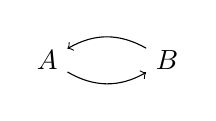
\begin{tikzpicture}
\node at (0,0) (A) {$A$};
\node (B) [right=of A] {$B$};
\path[->] (A) edge[bend right] node [right] {} (B);
\path[->] (B) edge[bend right] node [right] {} (A);
\end{tikzpicture}
\caption{Secret Santa protocol for 2 participants}
\label{fig:on}
\end{figure}


\begin{figure}[ht]
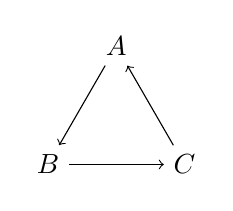
\begin{tikzpicture}
\node at (canvas polar cs:angle=90,radius=1cm) (A) {$A$};
\node at (canvas polar cs:angle=210,radius=1cm) (B) {$B$};
\node at (canvas polar cs:angle=330,radius=1cm) (C) {$C$};
\path[->] (A) edge node [right] {} (B);
\path[->] (B) edge node [right] {} (C);
\path[->] (C) edge node [right] {} (A);
\end{tikzpicture}
\qquad
\qquad
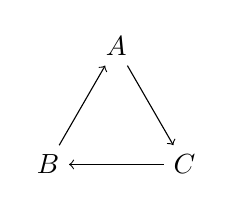
\begin{tikzpicture}
\node at (canvas polar cs:angle=90,radius=1cm) (A) {$A$};
\node at (canvas polar cs:angle=210,radius=1cm) (B) {$B$};
\node at (canvas polar cs:angle=330,radius=1cm) (C) {$C$};
\path[->] (B) edge node [right] {} (A);
\path[->] (C) edge node [right] {} (B);
\path[->] (A) edge node [right] {} (C);
\end{tikzpicture}
\caption{Secret Santa protocols for 3 participants; the two are the same up to reordering of participants}
\label{fig:tw}
\end{figure}


\begin{figure}[ht]
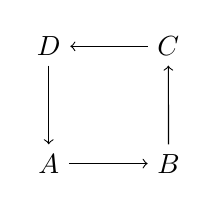
\begin{tikzpicture}
\node at (0,0) (A) {$A$};
\node (B) [right=of A] {$B$};
\node (C) [above right=of A] {$C$};
\node (D) [above=of A] {$D$};
\path[->] (A) edge node [right] {} (B);
\path[->] (B) edge node [right] {} (C);
\path[->] (C) edge node [right] {} (D);
\path[->] (D) edge node [right] {} (A);
\end{tikzpicture}
\qquad
\qquad
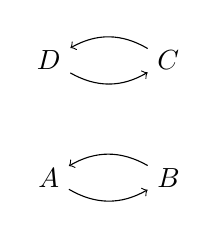
\begin{tikzpicture}
\node at (0,0) (A) {$A$};
\node (B) [right=of A] {$B$};
\node (C) [above right=of A] {$C$};
\node (D) [above=of A] {$D$};
\path[->] (A) edge[bend right] node [right] {} (B);
\path[->] (B) edge[bend right] node [right] {} (A);
\path[->] (C) edge[bend right] node [right] {} (D);
\path[->] (D) edge[bend right] node [right] {} (C);
\end{tikzpicture}
\caption{Secret Santa protocols for 4 participants (up to reordering of participants)}
\label{fig:th}
\end{figure}


Staring at these figures, a picture emerges:


\begin{prop}
Let $G$ be the graph of a Secret Santa protocol.
Then $G$ is composed of disjoint cycles.
\end{prop}

\begin{proof}
Pick a participant $x_1 \in G$.
The Secret Santa rules say there exists exactly one $x_2$ such that $x_1 \to
x_2$ and $x_2 \not= x_1$.
We keep extending the path this way until we get to an element $x_n$ that is
already in the path, that is, $x_n = x_m$ for some $1 \leq m < n$.
This must happen eventually because $G$ is finite.
We claim that $x_n = x_1$:
If not, that is if $x_n = x_m$ with $1 < m < n$, then we have
$$
\begin{tikzpicture}
\node at (canvas polar cs:angle=120,radius=1cm) (A) {$x_{m-1}$};
\node at (canvas polar cs:angle=0,radius=1cm) (B) {$x_m$};
\node at (canvas polar cs:angle=240,radius=1cm) (E) {$x_{n-1}$};
\path[->] (A) edge node [right] {} (B);
\path[->] (E) edge node [right] {} (B);
\end{tikzpicture}
$$
and the Secret Santa protocol implies that $x_{n-1} = x_{m-1}$.
But this contradicts our assumption that $x_m$ was the first element that
appeared twice in the path.
Therefore $x_1 \to x_2 \to \cdots \to x_n \to x_1$ is a cycle in $G$.
If there are any elements in $G$ that are not in this cycle, we pick one of
them and play the same game again until we have exhausted $G$.
\end{proof}


This result, felt in the bones of those who do not have the formal training to
state and prove it, is clearly the reason some people are not excited about the
office Secret Santa ritual.
How could they be?
A directed cycle is a trivial structure, having no exciting topology to speak of.
The heart desires action, drama, nontrivial homology; to live.



\subsection*{Counting Secret Santas}

The conditions the Secret Santa relation satisfies imply that it defines
a \emph{derangement} of $P$, that is, a permutation without fixed points.
The number of derangements of a set with $n$ members is known.
It is denoted by $!n$ and is given by the recursive formula
\[
!n = (n-1) (!(n-1) + !(n-2)), \quad n \geq 2,
\]
with $!0 = 1$ and $!1 = 0$.
There are many other ways to express this number. One is
\[
!n = n! \sum_{k = 0}^n \frac{(-1)^k}{k!}.
\]
The first few values of the sequence this defines are:
\[
\begin{tabular}{c|ccccccccc}
$n$ & 2 & 3 & 4 & 5 & 6 & 7 & 8 & 9 & 10
\\
\hline
$!n$ & 1 & 2 & 9 & 44 & 265 & 1854 & 14,833 & 133,496 & 1,334,961
\end{tabular}
\]
All are mere collections of disjoin cycles, as discussed above.


\section{Doing more, therefore better}

Reviewing the Secret Santa rules, they say that no person should give a gift to
themselves, and should give and receive exactly one gift.
As we have seen, this results in uninspiring Secret Santa graphs and the
degeneration of holiday cheer.
There is an obvious way of generalizing the classical Secret Santa protocol
that we now inspect.


\begin{defi}
Let $P$ be a finite set of participants and let $k$ be a positive
integer. A \emph{$k$-Secret Santa} protocol on $P$ is a relation on $P$
such that:
\begin{enumerate}
\item
If $x \in P$ there exist exactly $k$ different participants $y \in P$ such
that $x \sim y$.

\item
If $x \in P$ there exist exactly $k$ different participants $y \in P$ such
that $y \sim x$.

\item
No $x \in P$ satisfies $x \sim x$.
\end{enumerate}
\end{defi}

Each participant now gives and receives exactly $k$ gifts.
The case $k = 1$ is the classical Secret Santa protocol, and
the conditions on different participants imply that $k < |P|$.
Note that the case $k = |P| - 1$ means that each participant gives a gift to
everyone else.
This removes some of the uncertainty from Secret Santa (``I wonder who gave me
a gift?'') -- uncertainty which forms part of the core concept -- so we will not
consider this case further.

As before we can view a $k$-Secret Santa protocol as a directed graph $G$, which
we will call a $k$-Secret Santa graph.
Our conditions now say that each vertex in the graph has in- and out-degree
equal to $k$, and that no vertex is connected to itself.
Standard results on graphs then yield the following result, generalizing part
of our previous characterization of classical Secret Santa graphs.


\begin{prop}
Let $G$ be a $k$-Secret Santa graph. Then $G$ decomposes into a disjoint set of
graphs, each of which is spanned by an Eulerian cycle.
\end{prop}


Recall that classical Secret Santa also stipulates that the value of each gift
should not exceed $M$ monetary units.
In $k$-Secret Santa we should then either give gifts whose value does not
exceed $M / k$ monetary units, quickly resulting in the most trivial of gifts,
or spend up to $kM$ monetary units, soon adding significant strain on
household budgets in an already straining month.

We will thus restrict ourselves to the investigation of $2$-Secret Santa
protocols in what follows, leaving the analysis of higher Secret Santa
protocols to interested wealthier readers.





\end{document}
